\subsection{Компьютерное моделирование}
\label{sec:2b}

% TODO: Почему иридий?
Кластеры иридия моделировались при очень низких температурах. %TODO: Порядок температур
В таких условиях атомы иридия кристаллизуются преимущественно в гранецентрированные
и объемноцентрированные кристаллические решетки.

Начальная конфигурация нанокластера иридия строилась как фрагмент гранецентрированной
кристаллической решетки. Параметры, необходимые для расчета потенциала Саттона--Чена
для такой конфигурации, были опубликованы в \cite{kimura1998}
и приведены в таблице~\ref{table:iridium}.

\begin{table}[h!]
\begin{center}
\begin{tabular}{|c|c|c|c|c|c|}
\hline
 & m & n & $\epsilon$ & c & a \\
\hline
Ir & 6 & 13 & $3.7674\times10^{-3}$ & 224.815 & 3.83\\
\hline
\end{tabular}
\caption{Параметры модели Саттона-Чена для иридия}
\label{table:iridium}
\end{center}
\end{table}

В настоящей работе использовался конечно-разностный алгоритм решения уравнений ньютоновской динамики,
известный в англоязычной литературе как ``leapfrog algorithm''% \cite{Bargiel1991}.
Он представлен формулами:

\begin{equation}
\label{LF1}
\mathbf{p}^{n+1/2}_i = \mathbf{p}^{n-1/2}_i + \Delta t \, \mathbf{F}^{n}_i,
\end{equation}

Здесь $\mathbf{p_i}$ -- импульс i-го атома, n -- номер узла на временной шкале. Силы находятся дифференцированием полной потенциальной энергии системы как функции координат интересующего нас i-го атома:
\begin{equation}
\label{LF:Force}
\mathbf{F}^{n}_i = - \left(\dfrac{\partial {\Phi}^n}{\partial x^{n}_i}, \dfrac{\partial {\Phi}^n}{\partial y^{n}_i}, \dfrac{\partial {\Phi}^n}{\partial z^{n}_i} \right).
\end{equation}
Здесь
\begin{equation}
\dfrac{\partial {\Phi}^n}{\partial x^{n}_i} = \left. \dfrac{\partial \Phi}{\partial x_i} \, \right|_{\{\mathbf{r}_i\} = \{\mathbf{r}^{n}_i\}}.
\end{equation}

\begin{equation}
\label{LF2}
\mathbf{r}^{n+1}_i = \mathbf{r}^{n}_i + \Delta t \, \mathbf{p}^{n+1/2}_i/m_i,
\end{equation}

\begin{equation}
\label{LF3}
\mathbf{p}^{n}_i = \dfrac{1}{2} \left(\mathbf{p}^{n+1/2}_i +
\mathbf{p}^{n-1/2}_i \right),
\end{equation}

\begin{equation}
\label{LF4}
K^n = \dfrac{1}{2} \sum_{i} |\mathbf{p}^{n}_i|^2/m_i,
\end{equation}

\begin{equation}
\label{LF5}
E^n = {\Phi}^n + K^n .
\end{equation}
Как правило, временной шаг $\Delta t$ выбирается так, чтобы самый быстрый атом перемещался не более чем на $5\%$
межатомного расстояния $d$ \cite{Eckstein1991}:
\begin{equation}
\label{LF6}
\Delta t = 0.05 \, d \left( \dfrac{m_s}{2 K_s^n} \right)^{\frac{1}{2}}.
\end{equation}

Для каждого временного интервала (в каждом узле $n$) рассчитывается значение общей кинетической энергии $K^n$.
Если $K^n < K^{n-1}$, то есть был найден локальный максимум,
то все значения импульсов $p_{i}$ обнуляются, для того, чтобы уменьшить накопление общей погрешности в вычислениях.

Итерационный процесс заканчивается либо по достижении максимального количества итераций,
либо когда очередной локальный минимум кинетической энергии меньше порогового значения $\delta$.
При выполнении численных экспериментов максимальное количество итераций было равно $10000$,
а значение $\delta$ было равным $10^{-8}$.

Пример изменения значения кинетической энергии $K^n$ во времени изображен на
рис. \ref{kinet_energy_MD} и \ref{kinet_energy_MD_norm}.
Ось ординат на рис. \ref{kinet_energy_MD} масштабирована логарифмически.

\begin{figure}[h!]
\centering
  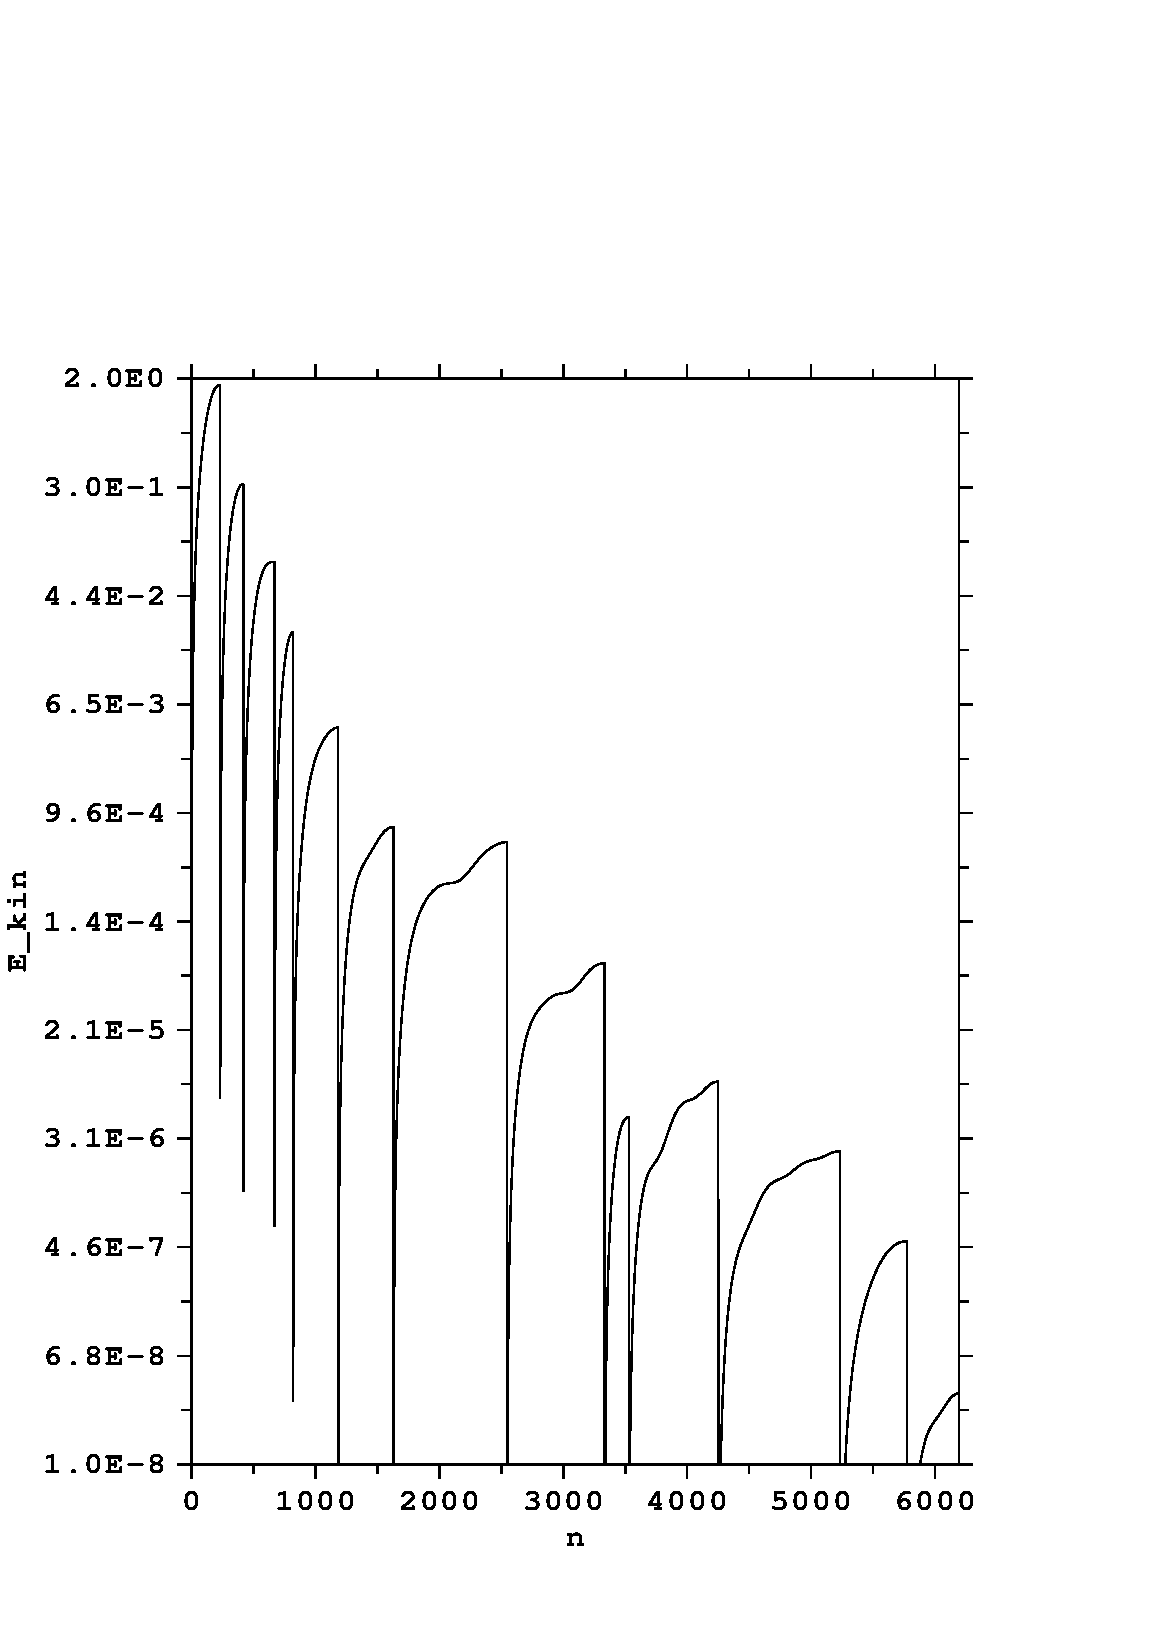
\includegraphics[width=1.0\textwidth]{./FIGs/Kin_energy_MD.pdf}
  \caption{Изменение кинетической энергии во времени (логарифмическое масштабирование)}
\label{kinet_energy_MD}
\end{figure}

\begin{figure}[h!]
\centering
  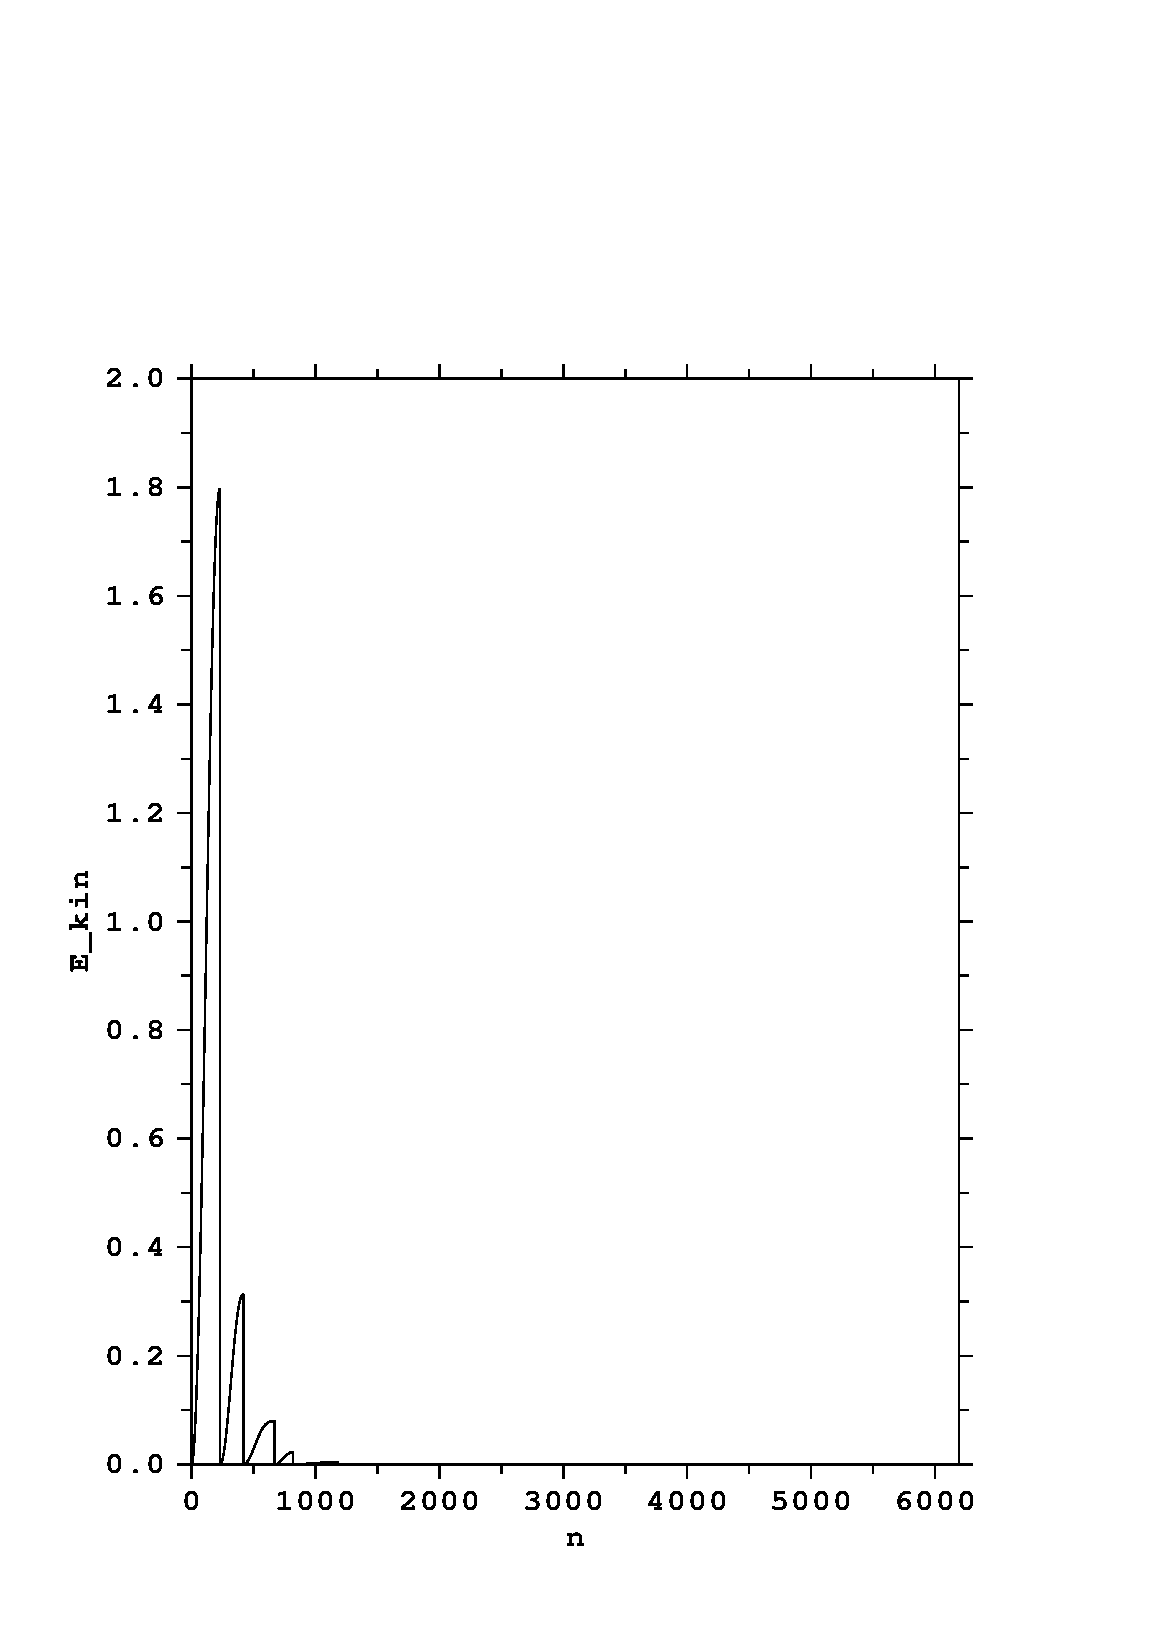
\includegraphics[width=1.0\textwidth]{./FIGs/Kin_energy_MD_norm.pdf}
\caption{Изменение кинетической энергии во времени}
\label{kinet_energy_MD_norm}
\end{figure}
